% Autor: Simon May
% Datum: 2017-10-05
% Diese Datei bietet ein minimalistisches Grundgerüst für ein LaTeX-Dokument,
% z.B. für die Bearbeitung der Aufgaben.
\documentclass[
	% Papierformat
	a4paper,
	% Schriftgröße (beliebige Größen mit „fontsize=Xpt“)
	12pt,
	% Schreibt die Papiergröße korrekt ins Ausgabedokument
	pagesize,
	% Sprache für z.B. Babel
	ngerman
]{scrartcl}

% Achtung: Die Reihenfolge der Pakete kann (leider) wichtig sein!
% Insbesondere sollten (so wie hier) babel, fontenc und inputenc (in dieser
% Reihenfolge) als Erstes und hyperref und cleveref (Reihenfolge auch hier
% beachten) als Letztes geladen werden!

% Silbentrennung etc.; Sprache wird durch Option bei \documentclass festgelegt
\usepackage{babel}
% Verwendung der Zeichentabelle T1 (Sonderzeichen etc.)
\usepackage[T1]{fontenc}
% Legt die Zeichenkodierung der Eingabedatei fest, z.B. UTF-8
\usepackage[utf8]{inputenc}
% Schriftart
\usepackage{lmodern}
% Zusätzliche Sonderzeichen
\usepackage{textcomp}

% Mathepaket (intlimits: Grenzen über/unter Integralzeichen)
\usepackage[intlimits]{amsmath}
% Ermöglicht die Nutzung von \SI{Zahl}{Einheit} u.a.
\usepackage{siunitx}
% Zum flexiblen Einbinden von Grafiken (\includegraphics)
\usepackage{graphicx}
% Abbildungen im Fließtext
\usepackage{wrapfig}
% Abbildungen nebeneinander (subfigure, subtable)
\usepackage{subcaption}
% Funktionen für Anführungszeichen
\usepackage{csquotes}
% Zitieren, Bibliographie
\usepackage{biblatex}

% Verlinkt Textstellen im PDF-Dokument
\usepackage[unicode]{hyperref}
% "Schlaue" Referenzen (nach hyperref laden!)
\usepackage{cleveref}

% siunitx: Deutsche Ausgabe, Messfehler getrennt mit ± ausgeben
\sisetup{
	locale=DE,
	separate-uncertainty
}

\begin{document}
\begin{titlepage}
	\centering
	{\scshape\LARGE Versuchsbericht zu \par}
	\vspace{1cm}
	{\scshape\huge XRAY \par}
	\vspace{2.5cm}
	{\LARGE Gruppe 6 Mo\par}
	\vspace{0.5cm}
	{\large Nils Kulawiak (E-Mail: n\_kula01@wwu.de) \par}
	{\large Oliver Brune (E-Mail: o\_brun02@wwu.de) \par}
	\vfill
	durchgeführt am 11.06.2018\par
	
	\vfill
	betreut von Christoph Angrick
	{\large \today\par}
\end{titlepage}

\tableofcontents
		
\newpage

\section{Einleitung}
\section{Methoden}
\label{Methode}
In diesem Versuch wurden verschiedene Eigenschaften von Röntgenstrahlung untersucht. Hierfür wurde eine Röntgenröhre mit Kupferanode verwendet. Der schematische Aufbau einer Röntgenröhre ist in \cref{roentgen} dargestellt.
\begin{figure}[h!]
	\centering
	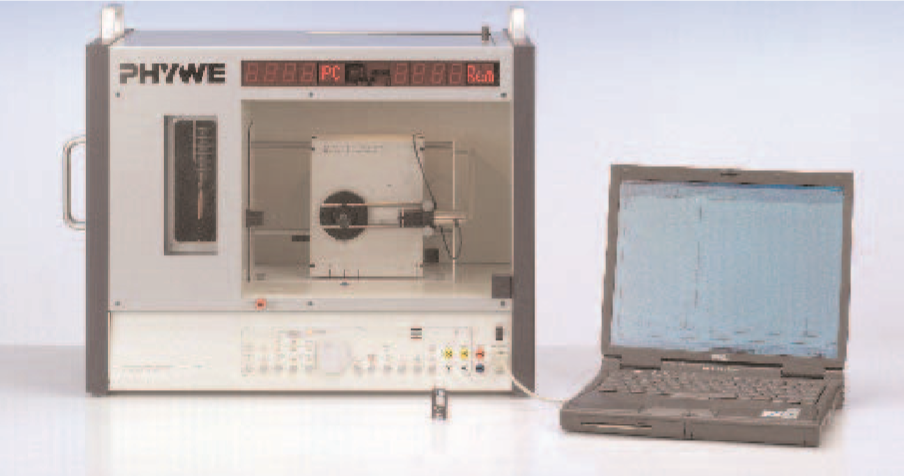
\includegraphics[scale = 1]{aufbau.png} %eigentlich röntgen.png aber hast vergessen das hochzuladen
	\caption{Schematischer Aufbau einer Röntgenröhre}
	\label{roentgen}
\end{figure}
In einem Gehäuse, in dem ein Vakuum herrscht, befinden sich Kathode und Anode der Röntgenröhre. Die Kathode besteht aus einem Metalldraht, oft Wolfram, der mit einer Heizspannung zum Glühen gebracht wird. Dadurch werden Elektronen aus dem Draht herausgelöst und bilden eine Elektronenwolke um den Draht. Wenn nun eine Anodenspannung angelegt wird (in diesem Versuch meist \SI{35}{kV}), dann werden die Elektronen in Richtung der Anode beschleunigt. In diesem Versuch besteht die Anode aus Kupfer. Treffen die hochenergetischen Elektronen auf das Kupfer, werden sie durch Wechselwirkung mit den Atomen abgebremst, es entsteht Bremsstrahlung mit einem kontinuierlichen Energiespektrum. Aus diesem Spektrum stechen allerdings bestimmte Energien deutlich heraus, die öfter erzeugt werden. Das sind die Röntgenstrahlen, die entstehen, wenn ein freies Elektron ein Elektron aus der K-Schale eines Kupferatoms ionisiert. Wenn das passiert, füllt ein Elektron aus der L- oder der M-Schale den freigewordenen Platz auf. Die Energiedifferenz zwischen den beiden Schalen gibt das Elektron dann in Form von Röntgenstrahlung ab. Die Linien im Energiespektrum sind dann gerade die so erzeugten Röntgenstrahlen. Diese sind atomspezifisch, daher nennt man diese Strahlung charakteristische Röntgenstrahlung.

Die Anode steht in einem $45$°-Winkel zum Elektronenstrahl, damit die Röntgenstrahlung möglichst in Richtung der Probe gerichtet ist. Die Strahlung wird anschließend von einer Blende kollimiert, damit nur nahezu parallele Strahlen auf die Probe treffen. Die Probe ist in diesem Experiment immer einer von zwei Kristallen, an denen Bragg-Reflexion durchgeführt wird. Der eine ist ein LiF-Einkristall, der andere ein KBr-Einkristall. An diesen findet Bragg-Reflexion statt, sodass je nach Einfallswinkel immer genau eine Wellenlänge die Bragg-Bedingung erfüllt, die dann reflektiert wird und von einem Geiger-Müller-Zählrohr detektiert wird. Um das gesamte Spektrum der Röntgenstrahlung abzutasten, muss daher der Kristallwinkel und damit auch der Detektorwinkel variiert werden. Der abgefahrene Winkelbereich war bei jedem Versuchsteil unterschiedlich. Der Winkel wurde in $0,1$°-Schritten variiert, gemessen wurde in jeder Einstellung $2$ Sekunden lang.

Da beim Geiger-Müller-Zählrohr bei jedem detektierten Photon eine vollständige Gasentladung stattfindet, gibt es einen kurzen Zeitraum, in dem keine weitere Strahlung detektiert werden kann. Dieses Zeitintervall bezeichnet man als Totzeit, sie beträgt bei dem verwendeten Zählrohr etwa $\SI{90}{\micro \second}$. Um die tatsächliche Anzahl an Teilchen zu bestimmen, die auftreten, wird \cref{eq:korr} verwendet. Dabei ist $\tau$ die Totzeit $N$ die korrigierte Impulsrate und $N_0$ die gemessene Impulsrate.
\begin{equation}
	N = \frac{N_0}{1 - \tau \cdot N_0}
	\label{eq:korr}
\end{equation}
Im zweiten Versuchsteil wurde untersucht, welchen Einfluss die Anodenspannung und die Anodenstromstärke auf die Intensität der charakteristischen Röntgenstrahlung von Kupfer hat. Es sollte experimentell überprüft werden, ob für die Intensität der Strahlung gilt:
\begin{equation}
	I_K = B I_A (U_A - U_K)^1,5
	\label{eq:ik}
\end{equation}
($I_A$ = Anodenstrom, $U_A$ = Anodenspannung, $B$ = konst. und $U_K$= Ionisierungspotential der K-Schale)
Hierfür wurde zuerst die Spannung konstant bei $35$kV gehalten und die Stromstärke in $0,1$mA-Schritten zwischen $0,1$mA und $1$mA variiert. Anschließend wurde die Stromstärke konstant bei $1$mA gehalten und die Spannung in $3$kV-Schritten zwischen $11$kV und $35$kV variiert. Gemessen wurde hier nur bei Kristallwinkeln zwischen $19$° und $24$°.

\section{Auswertung}
Zuerst wurde die Abhängigkeit der Intensität der K-Strahlung von der Stromstärke untersucht. Die Intensität entspricht der nach \cref{eq:korr} korrigierten Impulsrate. Dieser Zusammenhang ist in \cref{strom} dargestellt. Offensichtlich hängt die Intensität linear vom angelegten Anodenstrom ab. Dies bestätigt die Vorhersage nach \cref{eq:ik}. Die Steigung der $K_\alpha$-Linie ist dabei deutlich größer als die der $K_\beta$-Linie, was auch in allen anderen Versuchsteilen so gemessen wurde.

\begin{figure}[h!]
	\centering
	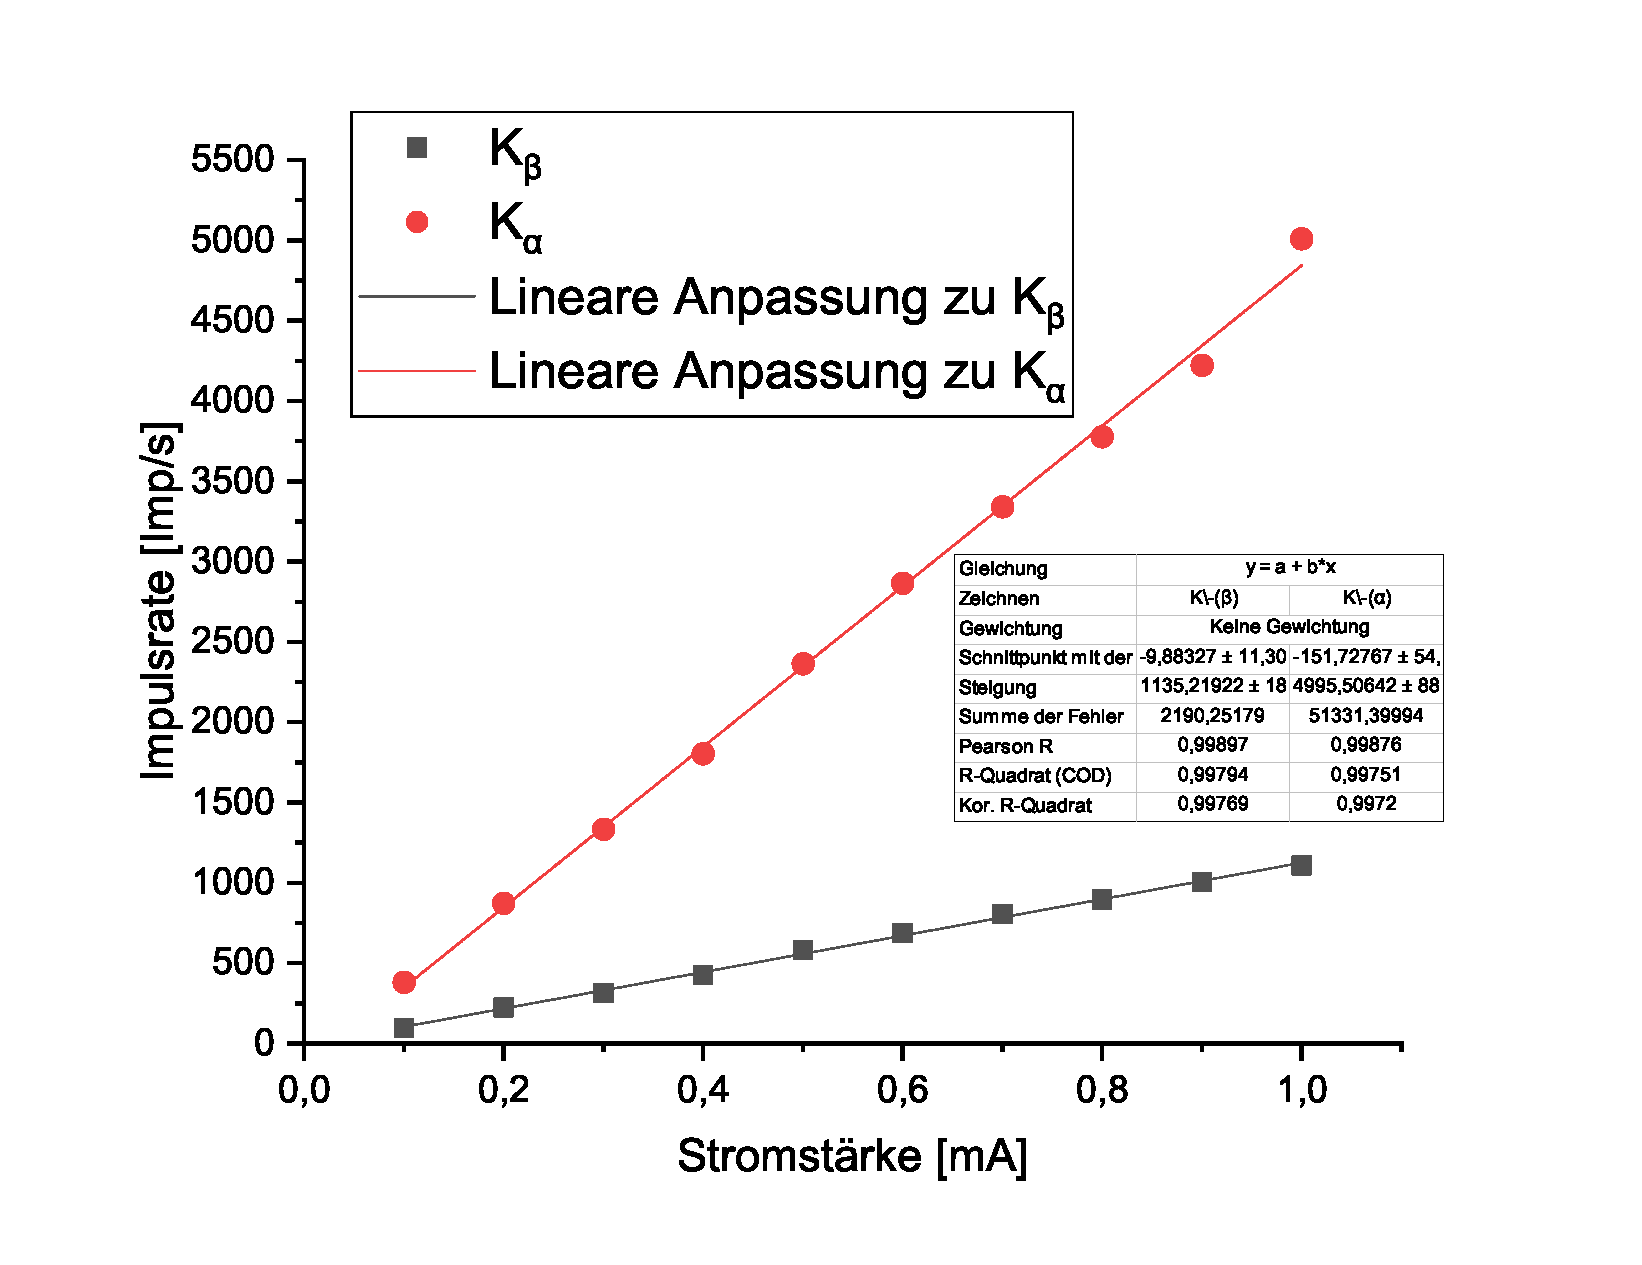
\includegraphics[scale = 0.6]{strom.eps}
	\caption{Die korrigierte Impulsrate aufgetragen gegen die angelegte Stromstärke. Der lineare Verlauf ist deutlich erkennbar.}
	\label{strom}
\end{figure}

Anschließend wurde der Einfluss einer Spannungsänderung auf die Intensität betrachtet. Auch hier entspricht die Intensität der nach \cref{eq:korr} korrigierten Impulsrate. Dieser Zusammenhang ist in \cref{spannung} dargestellt. Die Impulsrate steigt bei kleineren Spannungen erst langsam, bei höheren Spannungen aber immer stärker.

\begin{figure}[h!]
	\centering
	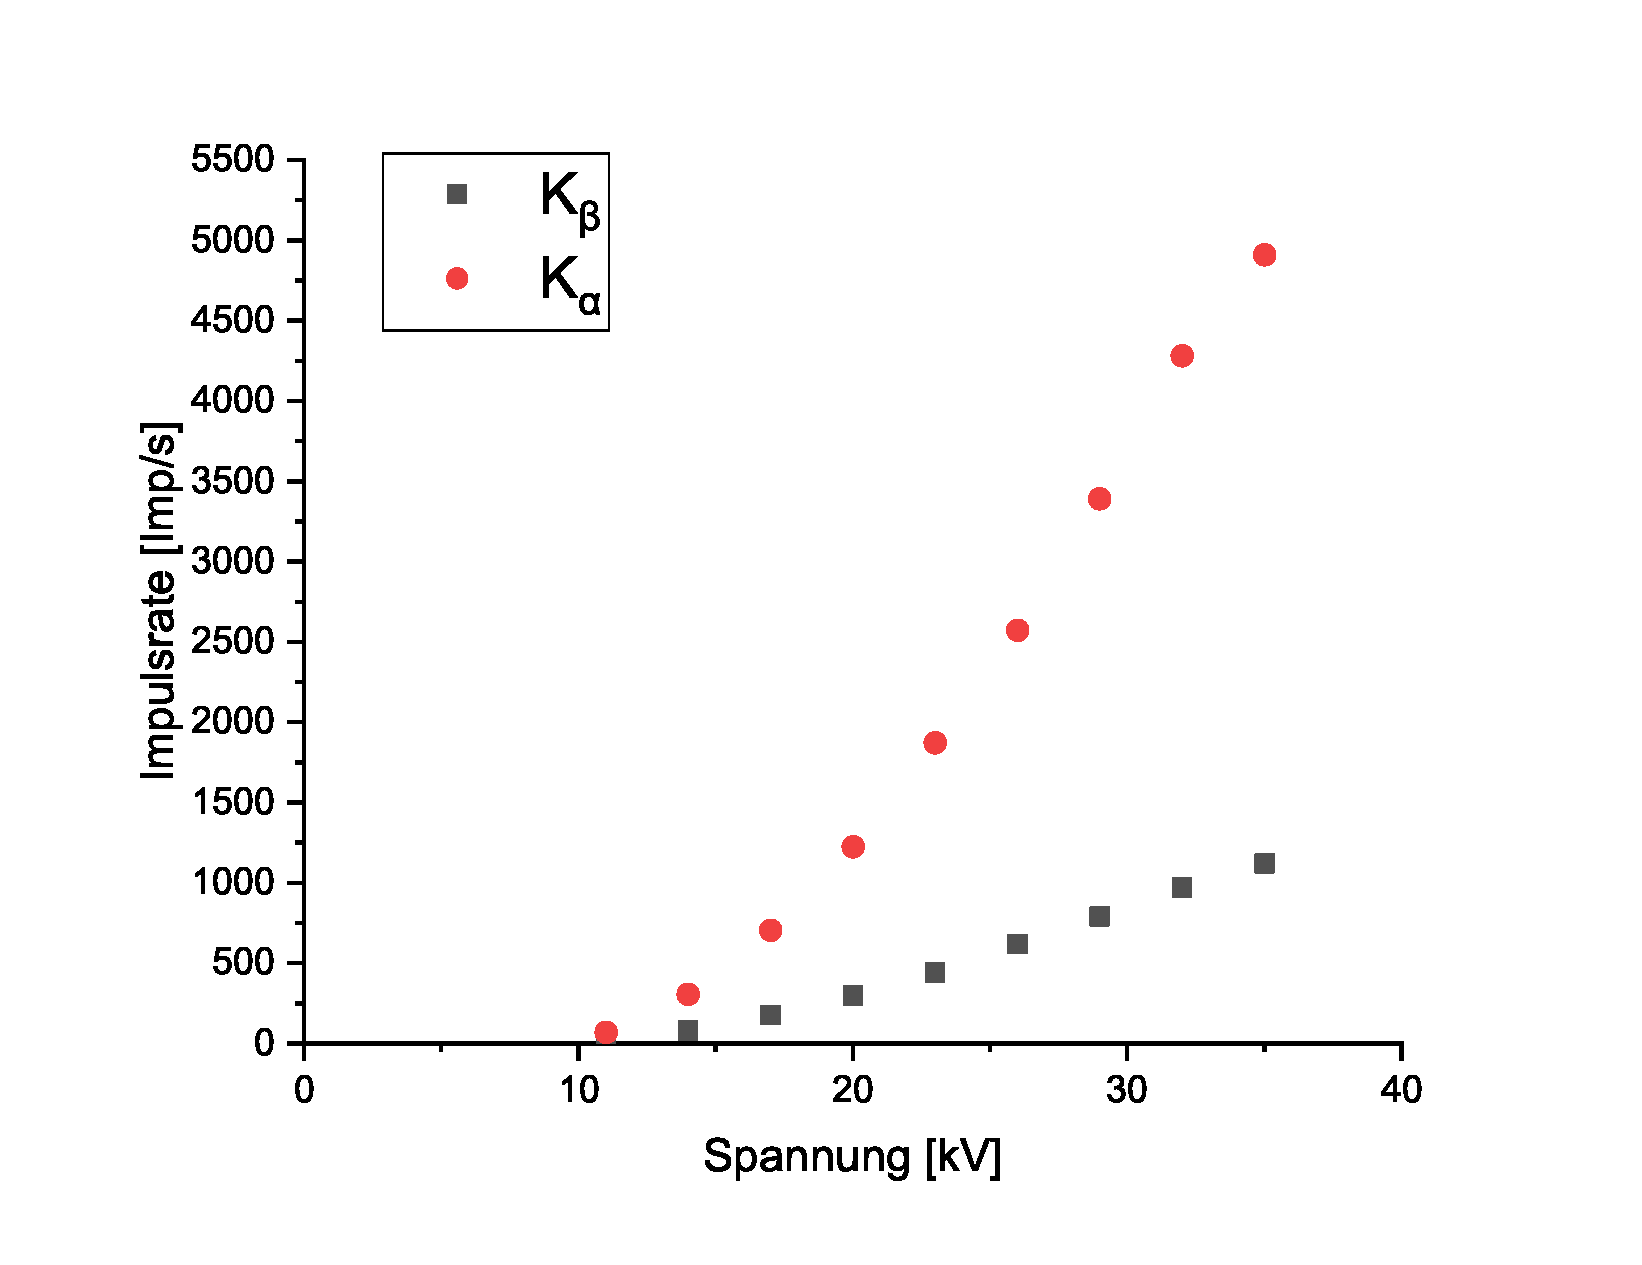
\includegraphics[scale = 0.6]{spannung.eps}
	\caption{Die korrigierte Impulsrate aufgetragen gegen die Spannung.}
	\label{spannung}
\end{figure}

 Um den in \cref{eq:ik} dargestellten Zusammenhang zu überprüfen, wurde in \cref{spannung2} die korrigierte Impulsrate gegen $(U_A - U_K)^{1,5}$ aufgetragen. Hier ist der lineare Verlauf der beiden K-Linien wieder deutlich erkennbar, so wie in \cref{eq:ik} vorhergesagt.
 
 Somit konnte in diesem Abschnitt die Gültigkeit der Formel für die K-Linien in Kupfer gezeigt werden.

\begin{figure}[h!]
	\centering
	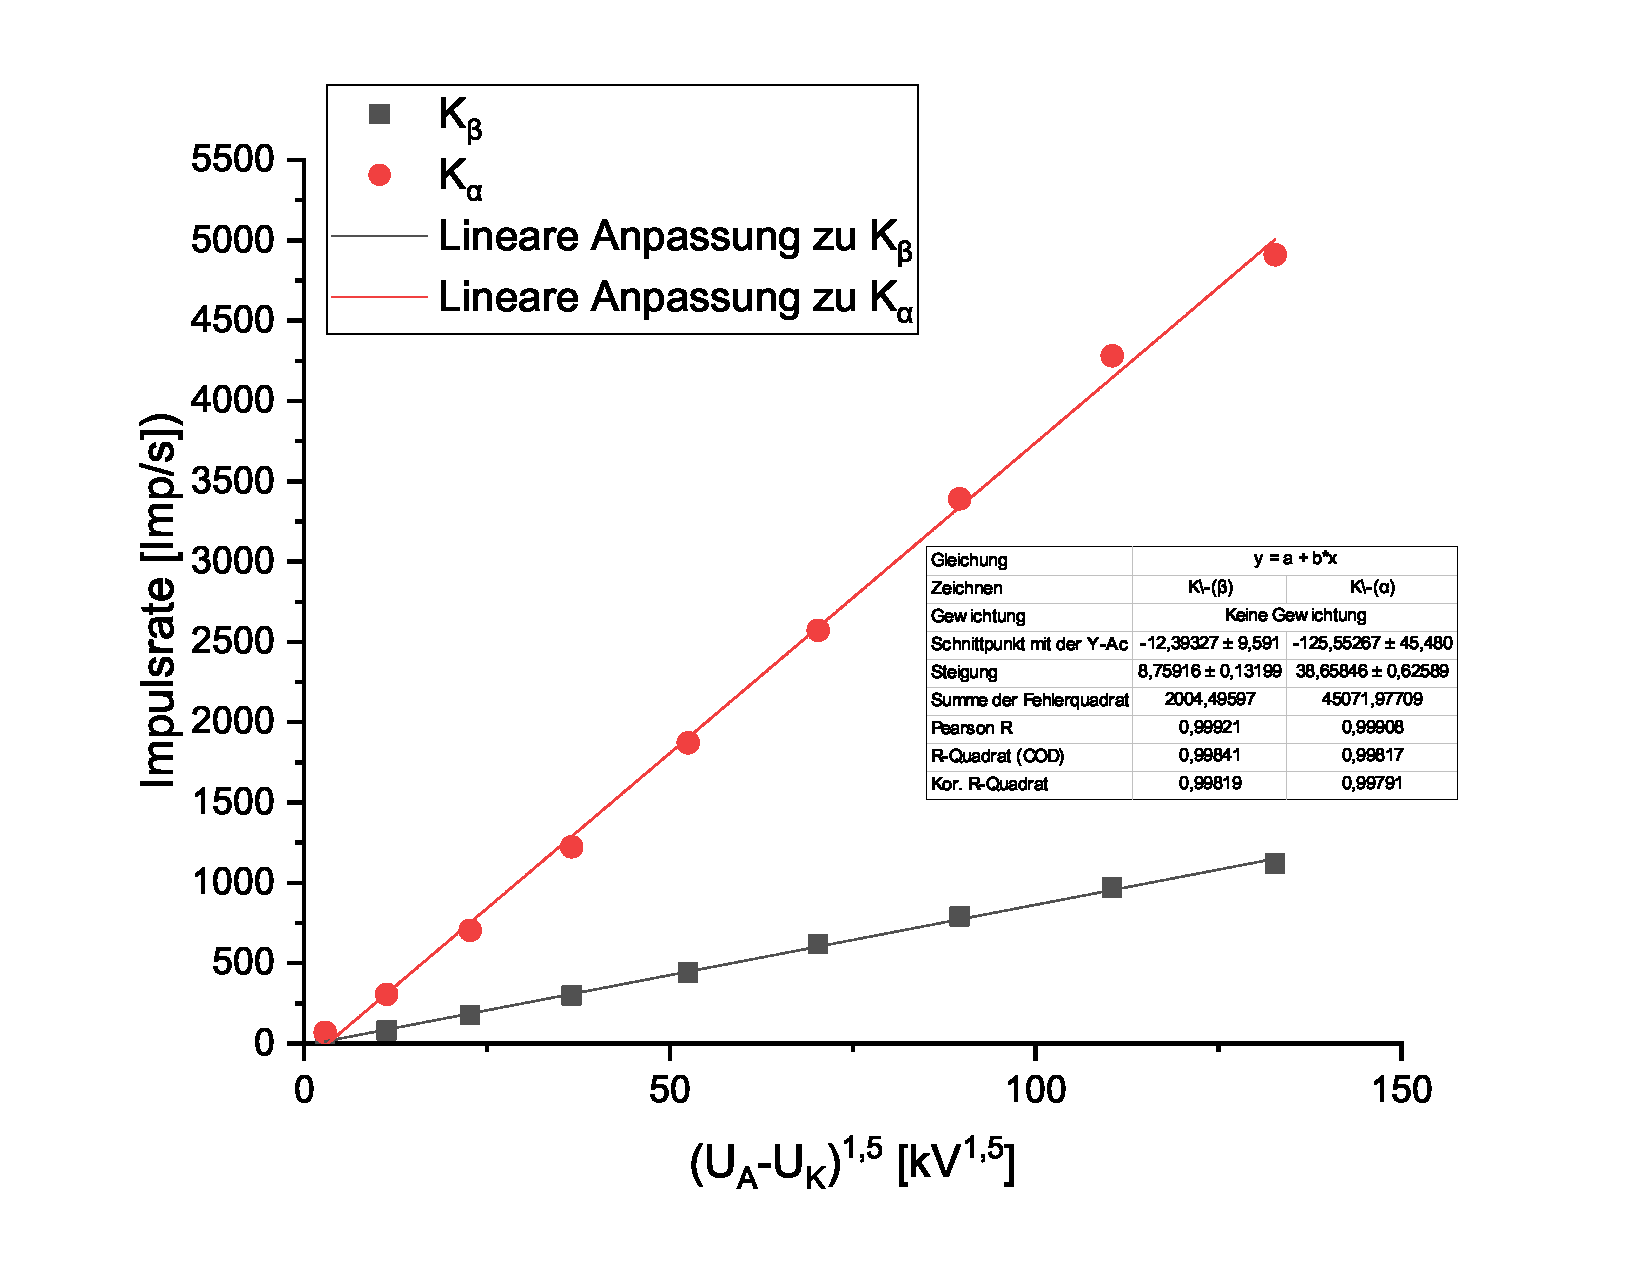
\includegraphics[scale = 0.6]{spannung2.eps}
	\caption{Die korrigierte Impulsrate aufgetragen gegen $(U_A-U_K)^{1,5}$. Der lineare Verlauf ist deutlich erkennbar.}
	\label{spannung2}
\end{figure}
In \cref{B1} ist der Aufbau zu sehen. In dem Kasten befindet sich eine Röntgenröhre. Das Charakteristische Material der Röntgenröhre ist Kupfer. Durch eine Blende kann die Röntgenstrahlung auf ein Analysator (in unserem Fall Kaliumbromid und Lithiumflourid) auftreffen und durch Bragg-Reflexion \cref{B2} auf einen Detektor (Geiger-Müller-Zählrohr) treffen. Diese Zählrate wird registriert und an einem Computer (rechts in \cref{B1}) dargestellt. Da das Geiger-Müller-Zählrohr eine Totzeit besitzt trifft mehr Strahlung ein als Registiert wird. Diese Korrektur ist in diesen Aufgabenteilen nicht nötig zu berücksichtigen, da für die Folgenden Auswertungen die Position der Maxima relevant ist und nicht deren Intensität.
\begin{figure}[h!]
    \centering
    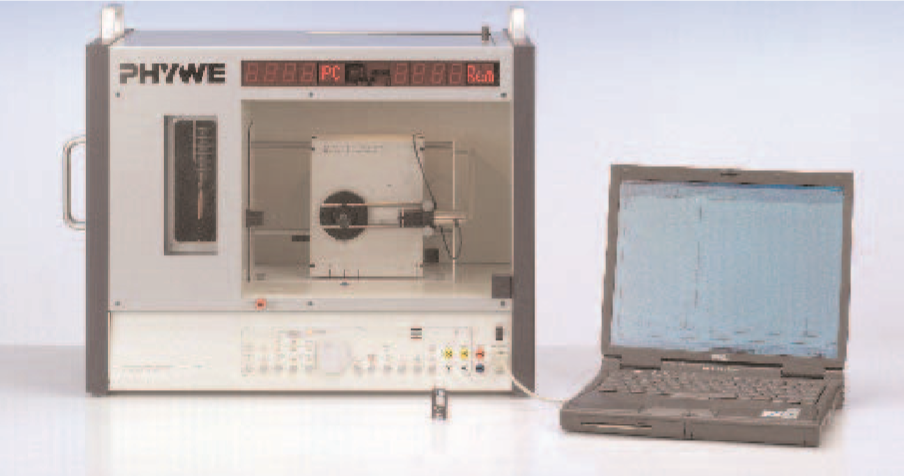
\includegraphics[scale = 1]{aufbau.png}
    \caption{}
    \label{B1}
\end{figure}
Um das Spektrum der Charakteristischen Strahlung der Anode qualitativ wird die Bragg-Bedingung benutzt. Diese kann durch \cref{B2} hergeleitet werden.
\begin{figure}[h!]
    \centering
    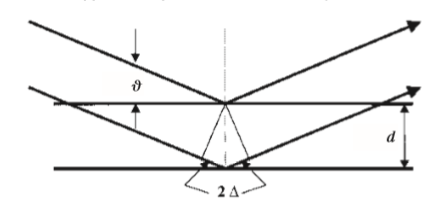
\includegraphics[scale = 1.5]{bragg.png}
    \caption{}
    \label{B2}
\end{figure}
Man erhält für die Energie 
\begin{align}
    E &= \frac{nhc}{2d\sin{\theta}} \cref{F1}
\end{align}
Dabei sind $\theta$ der Winkel und d der Abstand zwischen zwei Gitterebenen (hier sind die (200)-Ebenen die Ebenen an denen die Reflexe austeten), wie in \cref{B2} zu sehen. h und c sind das Plank'sche Wirkungsquantum und die Lichtgeschwindigkeit. n stellt die Anzahl der Perioden der Wellenlängen bei einer konstruktiven Interferenz dar.
Dadrurch können den entsprechenden Peaks eine Energie zugeordnet werden.
\begin{figure}[h!]
    \centering
    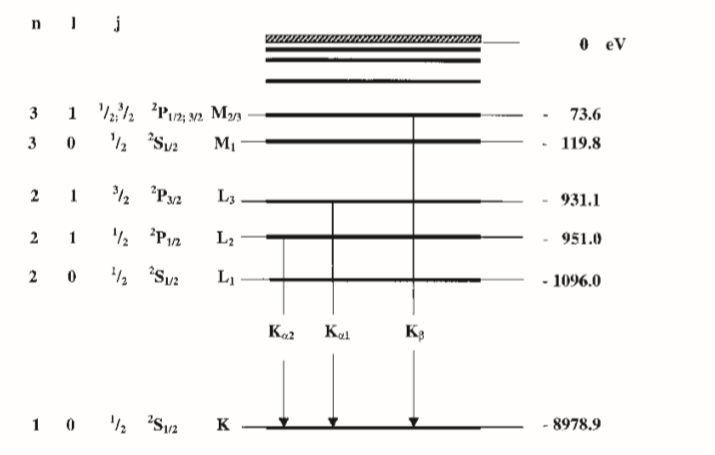
\includegraphics[scale = 1]{termschema.png}
    \caption{Hier ist das Thermschema einer Kupferanode dargestellt. Dabei sind die Relevanten Übergänge eingezeichnet.}
    \label{B3}
\end{figure}
Über \cref{B3} kann dann verglichen werden, ob die jeweiligen Übergänge zu Literaturwerten passt. Da die Auflösung nicht groß genug ist kann nicht zwischen einem $K_{\alpha1}$ und einem $K_{\alpha2}$ Zerfall unterschieden werden. Aus \cref{B3} kann für die einzelnen Zerfälle folgende Werte zugeordnet werden.
\begin{align*}
    K_{\alpha} &= 8,028 keV \\
    K_{\beta} &= 8,867 keV
\end{align*}
Als weitere Motivation wird gezeigt, wie ein Monochromatisches Spektrum erzeugt werden kann. Dafür gibt es zwei Methoden die erste Methode ist, indem der Kristall seine Richtung nicht ändert, die zweite Möglichkeit ist Monochromatisierung über Absorbtion zu erzeugen.

\section{Auswertung}
Zuerst wurden die verschiedenen Kennlinien aufgenommen. Dafür dient einmal ein Kaliumbromid(KBr)- und einmal ein Litiumfluoridkristall(LiF) als Analysator für die Energien der Kupferanode. Auf die Kupferanoden wurden die Elektronen mit einer Beschleunigungsspannung von 35keV beschleunigt. Das entspricht nach \cref{F1} einem Winkel im Spektrum von 3°. Bei späteren Versuchen wurde die Beschleunigungsspannung reduziert auf 25keV, sodass hier nur noch ein Winkel von 6° erreicht werden kann. Da die Netzenbenen für die beiden Kristalle bekannt sind und der Winkel aus \cref{A1} entnommen werden kann,
\begin{align*}
    d_{LiF} &= (2,014 \cdot 10^{-10})m \\
    d_{KBr} &= (3,290 \cdot 10^{-10})m  
\end{align*}
\begin{figure}[h!]
    \centering
    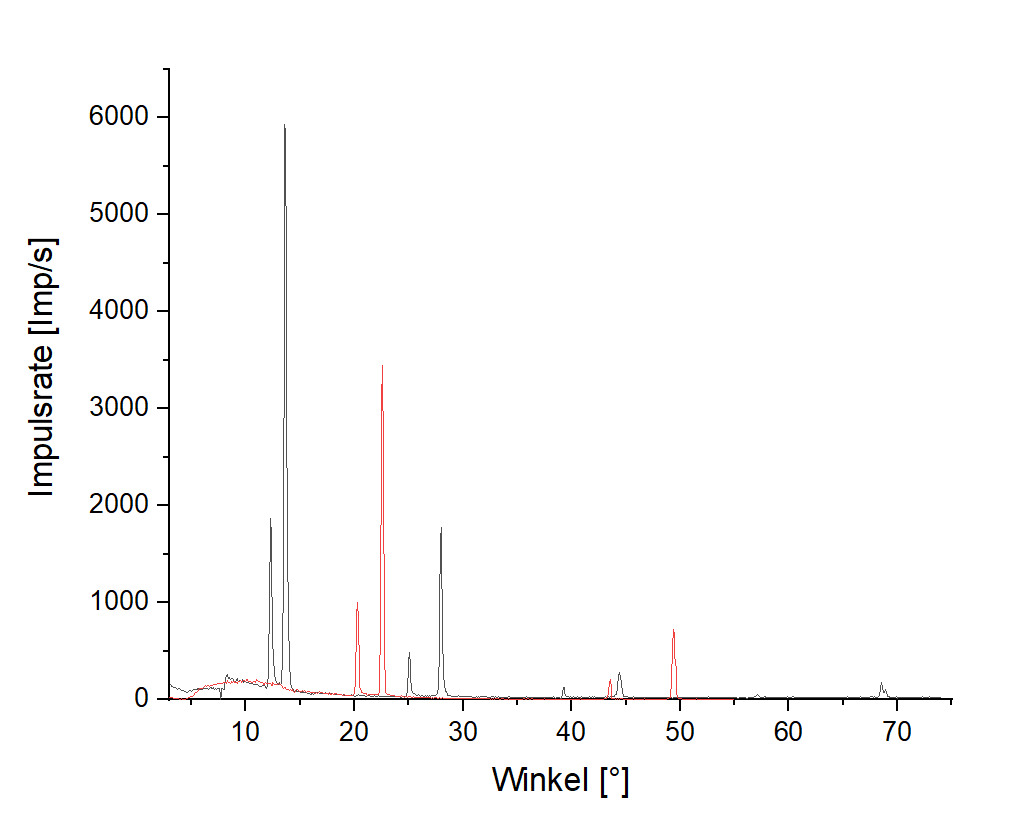
\includegraphics[scale = 0.6]{lif-kbr.png}
    \caption{Hier sind die Kennlinien einer Kupferanode mit einem Kaliumbromid Analysator(in schwarz) und einem Litiumfluorid Analysator(in rot) dargestellt.}
    \label{A1}
\end{figure}
kann für alle n ein Mittelwert der $K_{\alpha}$ und der $K_{\beta}$ Strahlung gezogen werden. Für den Mittelwert der Energien sind folgende Werte herausgekommen.
\begin{align*}
    K_{\alpha} &= (8,06 \pm 0,06) keV \\
    K_{\beta} &= (8,89 \pm 0,05) keV
\end{align*}

Als nächstes wurde dieselbe Messung mit einer Tubusblende mit einer Nickelfolie durchgeführt. Durch die Nickelfolie kam es zu einem geringen Intensitätsverlust der Strahlung. Da aber die Nickelfolie selbst einen Quantenübergang innerhalb der $K_{\alpha}$-Energie besitzt, werden diese Peaks wie in \cref{A3} bei Kaliumbromid und \cref{A4} bei Lithiumflourid zu sehen vollständig aufgehoben. Es bleiben nur noch die $K_{\beta}$-Energien übrig.
Somit kann nochmal die Energie der $K_{\beta}$ Strahlung bestimmt werden. 
\begin{align*}
    K_{\beta} &= (8,87 \pm 0,03)keV
\end{align*}
\begin{figure}[h!]
    \centering
    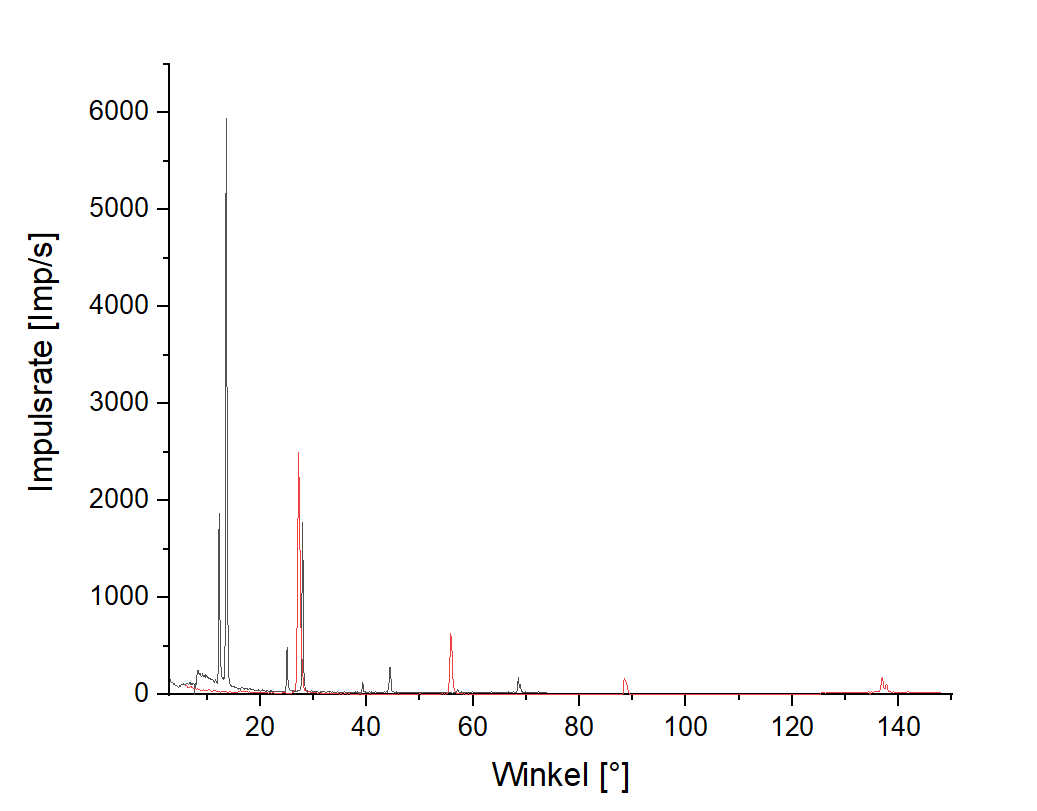
\includegraphics[scale = 0.6]{mono-normal.png}
    \caption{Hier sind die Kaliumbromid-Kurven aus \cref{A1} in schwarz und aus \cref{A2} in rot dargestellt.}
    \label{A3}
\end{figure}
\begin{figure}[h!]
    \centering
    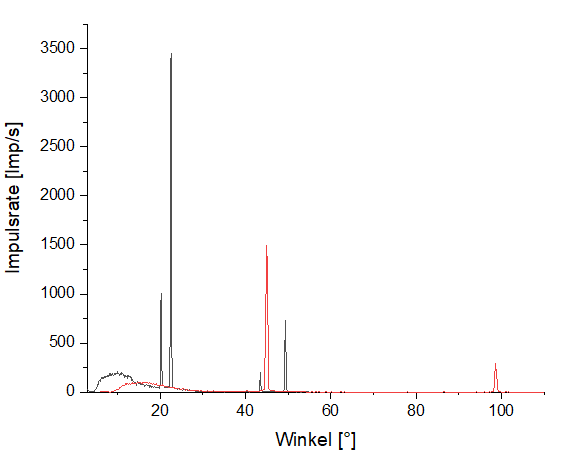
\includegraphics[scale = 1]{mono-norlif.png}
    \caption{Hier sind die Lithiumflourid-Kurven aus \cref{A1} in schwarz und aus \cref{A2} in rot dargestellt.}
    \label{A4}
\end{figure}
In diesem Teil wurde die Monochromatisierung dargestellt. Einmal bzgl. einem stationären Analysator, was in \cref{A6} gezeigt wird. Hier ist logisch, dass Monochromatisches Licht an der Detektorstelle entsteht, da jede andere Strahlung kein Reflex an dieser Gitterebene besitzt.
\begin{figure}[h!]
    \centering
    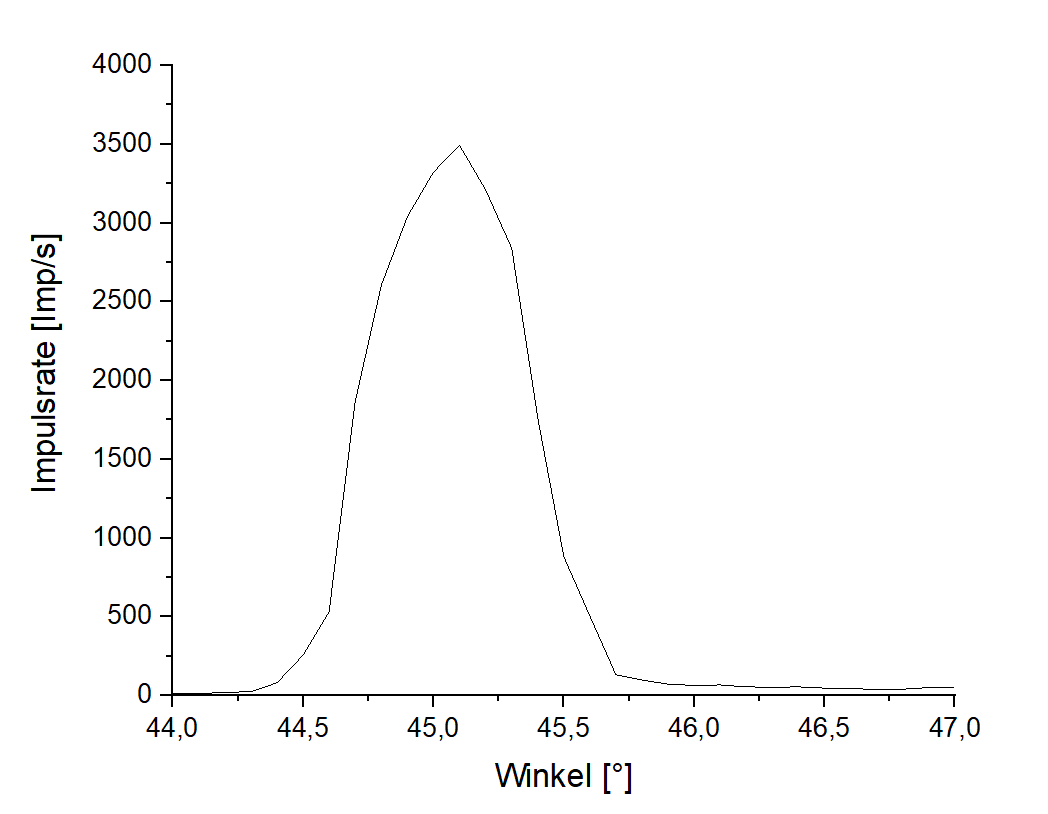
\includegraphics[scale = 0.6]{fest.png}
    \caption{Hier ist die Monochromatisierung dargestellt über das Verfahren, dass der der Analysator fix gehalten wird.}
    \label{A6}
\end{figure}
In zweiten Fall wurde eine Nickelfolie zwischen Detektor und Analysator positioniert, sodass hier an \cref{A7} erkannt werden kann, adss ebenfalls eine Monochromatisierung eintritt, in diesem Bereich des Spektrums, da wie bereits oben erwähnt, die $K_{\alpha}$ Strahlung im Nickel einen Quantensprung hervorruft und somit der Peak verschwindet.
\begin{figure}[h!]
    \centering
    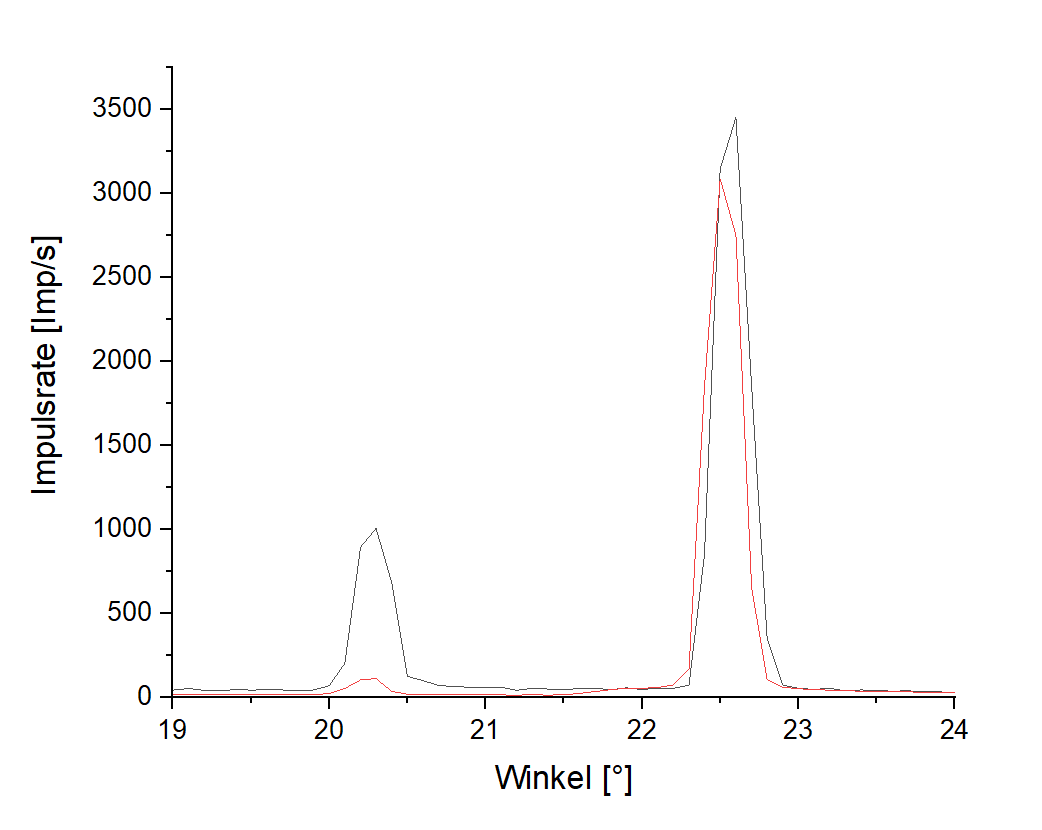
\includegraphics[scale = 0.6]{abs-mono.png}
    \caption{Hier ist die Monochromatisierung dargestellt über das Verfahren, dass Zwischen Analysator und Detektor ein Nickelfilter zwischengeschaltet wurde. In Rot ist die Monochromatisierte Kurve dargestellt und in Schwarz die Lithiumflourid-Kurve aus \cref{A1}.}
    \label{A7}
\end{figure}

\section{Unsicherheiten}
Die Unsicherheit des Winkel wo der Peak liegt wurde durch die Breite der Peaks abgeschätzt. Die Breite der Peaks nach beiden Seiten hinweg wurde auf $0,2$° geschätzt. Sodass sich eine Unsicherheit des Winkels durch die Dreickswahrscheinlichkeitssichtefunktion und der Umrechnung von Grad in Bogenmaß zu $0,0014$ Rad ergeben hat.
Die Unsicherheiten der Bragg-Gleichung wurden durch Fehlerfortpflanzung bestimmt, wobei die einzige Unsicherheitsquelle im Bogenmaß war.

\section{Diskussion}
Die Literaturwerte der Strahlungsarten lagen bei:
\begin{align*}
    K_{\alpha} &= 8,028 keV \\
    K_{\beta} &= 8,867 keV
\end{align*}
Die berechneten Werte anhand der Analysatorkristalle haben Werte von
\begin{align*}
    K_{\alpha} &= (8,06 \pm 0,06) keV \\
    K_{\beta} &= (8,89 \pm 0,05) keV
\end{align*}
ergeben, die in Betrachtung zu den Messunsicherheiten genau den Literaturwerte entsprechen. Duch die Filterung der $K_{\alpha}$ Linien konnte ein weiterer Wert für 
\begin{align*}
    K_{\beta} &= (8,87 \pm 0,03)keV
\end{align*}
ermittelt werden, der ebenfalls in hinblick auf die Messunsicherheiten genau zu den Literaturwerten passt.





\section{Absorptionsgesetz für Röntgenstrahlung}
\subsection{Methode}
Der Aufbau ist bis auf kleine Unterschiede analog zu \cref{Methode}. In diesem Fall wird für alle Versuchsteile eine Anodenspannung von 25kV angelegt. Außerdem wird hinter dem LiF-Kristall jeweils ein Absorber eingesetzt, welcher in diesem Teil des Versuchs hauptsächlich untersucht wird. In ersten Teil wird dabei Zink und Aluminium benutzt,wobei jeweils die Dicke der Absorber variiert wird und die verschiedenen Intensitäten verglichen werden, um den Absorptionskoeffizienten zu bestimmen. 

Im zweiten Teil wird Nickel betrachtet, welches nach der Absorptionskante untersucht wird, wobei jeder Winkel 50s lang gemessen wird, um eine möglichst genaue Auflösung zu erhalten.

Außerdem ist die Messung des LiF-Kristalls ohne Absorber benötigt.
\subsection{Auswertung}
\subsubsection{Absorptionskoeffizient Zink und Aluminium}

 Wenn Röntgenstrahlung auf ein Material trifft, kann der Absorptionskoeffizient berechnet werden mit
\begin{equation}
I = I_{0} e^{- \mu(\lambda,z) d}.
\label{Absorp}
\end{equation}

\begin{figure}[h!]
	\centering
	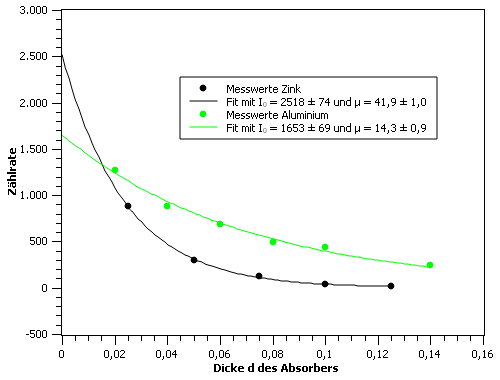
\includegraphics[scale = 1]{expo.png} 
	\caption{Exponentieller Abfall der Strahlung in Absorbern bei $\lambda$ = \SI{154,1}{pm}}
	\label{expo}
\end{figure}

Es wurde allerdings nicht der Wert in \cref{expo} für d=0 nicht benutzt, da er mit $I_{0} = 7523,6$ zu groß sind als das ein sinnvoller Fit noch möglich wäre, was darauf hindeutet, dass es zu einem Fehler bei der Messung kam, wie es später auch noch in \cref{Ni} sichtbar wird.

Außerdem soll der Zusammenhang näherungsweise gelten:
\begin{equation}
\dfrac{\mu}{\rho} = k(\lambda^{3} \cdot Z^{3}),
\label{Z}
\end{equation}
wobei k eine Konstante ist. Mit den Dichten für $\rho_{Al} = \SI{2,17}{\dfrac{g}{cm}}$ und $\rho_{Zn} = \SI{7,14}{\dfrac{g}{cm}}$ ergeben sich die Massenabsorptionskoeffizienten $\left(\dfrac{\mu}{\rho}\right)_{Al} = \SI{2,0 \pm 0,1}{\dfrac{cm^{2}}{g}}$ und $\left(\dfrac{\mu}{\rho}\right)_{Zn} = \SI{19,3 \pm 0,5}{\dfrac{cm^{2}}{g}}$. Da Zink eine Ladung von Z = 30 und Aluminium von Z = 13 hat, folgt daraus, dass der Quotient der beiden Massenabsorptionskoeffizienten ungefähr 12,3 groß sein sollte. In diesem Fall ergibt sich allerdings ein Quotient von 9,6.

\subsubsection{Absorptionskante Nickel}
\label{Ni}
Ziel ist es durch die Absorptionskante das Energieniveau der K-Schale zu bestimmen. Dafür wird in \cref{Kante} die Dritte Wurzel des Massenabsorptionskoeffizienten gegen die Wellenlänge der Strahlung aufgetragen. Der Massenabsorptionskoeffizient wird dabei wieder mithilfe von \cref{Absorp} berechnet und danach durch die Dichte von Nickel mit $\rho = \SI{8,99}{\dfrac{g}{cm^{3}}}$ geteilt. Diesmal werden allerdings nur zwei Werte pro Winkel benutzt.

Die Wellenlänge der Röntgenstrahlung folgt aus der Bragg-Bedingung mit
\begin{equation}
n \lambda = 2 d \sin(\theta),
\end{equation}
wobei n = 1 angenommen wird da das erste Maximum überwiegt. Die Absorptionskante entspricht dem Energieniveau, da es an diesem Punkt zur Ionisation der K-Schale kommen kann und somit der Absorptionskoeffizient mit höherer Energie bzw. niedrigerer Wellenlänge stark ansteigt. Aus dem linearen Fit in \cref{Absorp} lässt sich dann die Wellenlänge der Strahlung an der Absorptionskante bestimmen. Diese beträgt $\lambda_{k} = \SI{150,0 \pm 23,7}{pm}$. Die Unsicherheit folgt alleine aus dem linearen Fit, scheint aber unnötigerweise groß zu sein. Die Energie der K-Schale lässt sich daraufhin mit $E_{k} = \dfrac{h \cdot c}{\lambda_{k}} = \SI{8267 \pm 1303}{eV}$ berechnen. Dies stimmt auch mit dem Literaturwert von $E_{k} = \SI{8,33}{keV}$ gut überein.


\begin{figure}[h!]
	\centering
	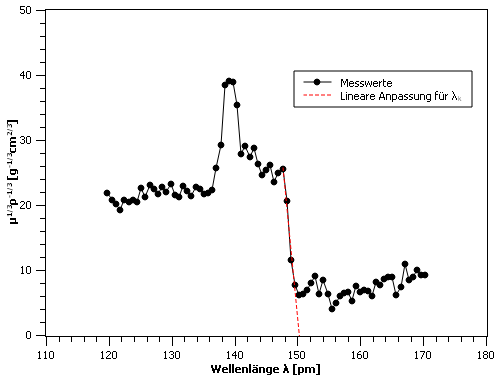
\includegraphics[scale = 1]{Absorptionskante.png}
	\caption{Absorptionskante von Nickel}
	\label{Kante}
\end{figure}

\subsection{Diskussion}
Im ersten Teil der Untersuchung von Absorbern sollte der Absorptionskoeffizient berechnet werden. Ein Problem dabei war allerdings, dass der Wert bei d=0 nicht benutzt werden konnte, weshalb der Fit wesentlich ungenauer wird. Das lässt sich auch daran erkennen, dass die Amplituden $I_{0}$ in \cref{expo} sich deutlich voneinander unterscheiden, obwohl das für beide Funktionen der gleiche Wert sein sollte. Trotzdem scheinen sich die Absorptionskoeffizienten zumindest in der richtigen Größenordnung zu befinden, wie auch der Vergleich mit der empirischen Funktion \cref{Z} zeigt.

Bei der Untersuchung von Nickel lies sich die Energie der k-Schale mit $E_{k} = \SI{8267 \pm 1303}{eV}$, die auch mit dem Literaturwert von $E_{k} = \SI{8,33}{keV}$ gut übereinstimmt, problemlos bestimmen. Allerdings sind die Werte in \cref{Kante} allesamt um einen Faktor von 4-10 größer, als in der Vorlage, was auf einen Fehler hinweisen könnte, was auch mit dem viel zu hohen Wert aus dem ersten Teil übereinstimmt. Höchstwahrscheinlich kommt dies durch einen Fehler in des Messung, wie z.B. unterschiedliche Blenden bei den verschiedenen Messungen. Trotzdem stimmt sowohl die grundlegende Form, als auch der Endwert mit den Literaturwerten überein. 
\begin{thebibliography}{9}
\bibitem{A}
Phywe Schriftenreihe Handbuch Physik,Experimente mit Röntgenstrahlen,PHYWE SYSTEME GMBH \& Co.KG , D-37070 Göttingen
 \end{thebibliography}
\end{document}
